\chapter{Models and control}
%http://tex.stackexchange.com/questions/13933/drawing-mechanical-systems-in-latex
In this chapter the derivative of the models used for this project is described. Furthermore the controller implemented will be described after the models has been introduced. The overview of the control system is shown on \figref{control_block} and \figref{fig:simple_control}  \todo{We need a another introduction.}

\input{rapport/Control/control_system_tikz}
\todo{elaborate on the block diagram}

\begin{figure}[H]
	\includegraphics[width=\textwidth]{rapport/pictures/control.pdf} 
	\caption{Simplified block diagram of the control design.}
	\label{fig:simple_control}
\end{figure}

\section{Human model}
In this section a model of a human arm and hand are derived. This is done because of the \todo{Need something for this}..
%ref
% http://research.vuse.vanderbilt.edu/cim/pubs/journal/13%20-%20Speich%20Shao%20and%20Goldfarb%202005.pdf

The human model can be describe from a mass-spring-damper model\todo{reference}, see figure \todo{figref}. This model has the base position in armpit of the operator. The constants $K_2$, $b_2$ and $K_1$, $b_1$ are the damper and spring constant for the arm and hand respectively. The mass, M, is the arm of the operator and the force, F, is the force between the hand and the manipulator, in this case the Geomagic touch.

\begin{figure}[H]
\centering
\begin{tikzpicture}[every node/.style={draw,outer sep=0pt,thick}]




\node (MO) [minimum width=1cm, minimum height=2.5cm] at (-3,0) {};
\node (M) [minimum width=1cm, minimum height=2.5cm] at (0,0) {$m_h$};

\draw [spring] ([yshift=0.7cm]MO.east) -- ([yshift=0.7cm]M.west);
\draw [damper] ([yshift=-0.7cm]MO.east) -- ([yshift=-0.7cm]M.west);

\node (wall) [ground, rotate=90, minimum width=3cm] at (3,0) {};
\draw (wall.north east) -- (wall.north west);

\draw [spring] ([yshift=0.7cm]M.east) -- ([yshift=0.7cm]wall.north);
\draw [damper] ([yshift=-0.7cm]M.east) -- ([yshift=-0.7cm]wall.north); %rotation makes the north, south, east and west rotate!

\draw [->,ultra thick] (-4.9,0) -- (-3.7,0);


\end{tikzpicture}
\caption{Simple human arm/hand dynamical model.}
\end{figure}
\todo{add b,K,F and mx and mh direction}




From \todo{figure} the dynamic equations can be derived as \eqref{eq:force_endo_hand2} and \eqref{eq:force_endow_hand}.

\begin{equation}
F_h = k_1(x_m-x_h)+b_1(x_m-x_h)s
\label{eq:force_endo_hand2}
\end{equation}

\begin{equation}
m_hx_hs^2 = k_1(x_m-x_h)+b_1(x_m-x_h)s-k_2x_h-b_2x_hs
\label{eq:force_endow_hand}
\end{equation}

By substituting the equations into each other the transfer function for the dynamic model can be found. In this case the transfer function is made for the force between the hand and the Geomagic touch and its position, see \eqref{eq:force_endo_hand3}

\begin{equation}
\frac{x_m}{F_h} = \frac{m_hs^2+(b_2+b_1)s+(k_2+k_1)}{m_hb_1s^3+(m_hk_1+b_1b_2)s^2+(k_1b_2+b_1k_2)s+k_2k_1}
\label{eq:force_endo_hand3}
\end{equation}
\section{Friction model}

The effort measured on the sbRIO is equal to the sum of the force required to overcome friction and the external forces applied to the end-effector. For the system to be transparent, the force required to overcome friction should not be fed back as this force would not be felt if the teleoperator was holding the tool directly. In order to isolate the external forces a friction model is required. The model built is based on the one described in \cite{force_reflection}. The total friction acting on an actuator can be divided as:
\todo{argue that we want a model of endo + motor and not 1 for each}
\begin{equation}
\tau_f = \tau_v + \tau_c + \tau_s
\label{eq:total_friction}
\end{equation} 

with:\\
\hspace*{8mm} $\tau_v$ viscous friction\\
\hspace*{8mm} $\tau_c$ coulomb friction\\
\hspace*{8mm} $\tau_s$ static friction    


The viscous friction is proportional to the opposite of the velocity:
\begin{equation}
\tau_v = F * w;
\label{eq:viscous_friction}
\end{equation}
with:\\
\hspace*{8mm}$w$ the angular velocity\\
\hspace*{8mm}$F$ a negative coefficient\\

The coefficient $F$ can be computed from the measurements made on the setup by plotting the effort depending on the velocity.

The stiction is the amount of effort required for the object to start moving when its velocity is zero. As such it can be described as:

\begin{equation} 
\tau_s =  \begin{cases} K_s, & \mbox{if } w = 0 \\ 0, & \mbox{else} \end{cases}
\label{eq:static_friction}
\end{equation}
with:\\
\hspace*{8mm}$w$ the angular velocity\\
\hspace*{8mm}$K_s$ a constant\\

The constant $K_s$ can be measured by increasing the current supplied to the motor until it starts moving. 
The coulomb friction occurs as a constant force opposing the movement:

\begin{equation}
\tau_c = sign(w)*K_c;
\label{eq:coulomb_friction}
\end{equation}
with:\\
\hspace*{8mm}$w$ the angular velocity\\
\hspace*{8mm}$K_c$ a constant determined experimentally\\
\hspace*{8mm}the $sign$ function is defined as $sign(w) = \begin{cases} 1, & \mbox{if } w > 0 \\ 0, & \mbox{if } w == 0 \\ -1, & \mbox{if } w < 0\end{cases}$\\

The constant $K_c$ can be measured by setting the motor in motion and decreasing the current until the motor stops moving.
From \eqref{eq:viscous_friction} to \eqref{eq:coulomb_friction}, the total friction given by \eqref{eq:total_friction} can be plotted as:

\begin{figure}
\centering
	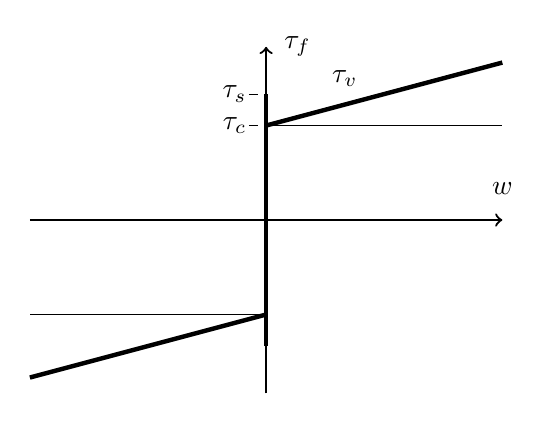
\begin{tikzpicture}
	\draw [->,thick] (-3,0) -- (3,0);
	\draw [->,thick] (0,-2.2) -- (0,2.2);
	\draw [ultra thick] (0,-1.6) -- (0,1.6);
	\draw [ultra thick] (0,1.2) -- (3,2);
	\draw [ultra thick] (0,-1.2) -- (-3,-2);
	\draw (0,1.2) -- (3,1.2);
	\draw (0,-1.2) -- (-3,-1.2);

	\node at (-0.4,1.6) {$\tau_s$};
	\draw (-0.22,1.6) -- (-0.1,1.6);
	\node at (-0.4,1.2) {$\tau_c$};
	\draw (-0.22,1.2) -- (-0.1,1.2);
	\node at (1,1.8) {$\tau_v$};


	\node at (3,0.4) {$w$};
	\node at (0.4,2.2) {$\tau_f$};

	\end{tikzpicture}
\caption{friction}
\end{figure}

\section{Embedded control system}

It is imperative to create a controller which minimizes the effects of communication delay. Therefore the aim was to implement as much of the motion control on the embedded system as possible. The human operator  inputs the required position by moving the GT. These positions are sent as position reference to the sbRIO. 
The sbRIO has an implemented cascade position-speed-current control, which takes care of the EndoWrist positioning tasks. The P position control that tracks the setpoint is running on the sbRIO FPGA. The FPGA sends the speed reference to the Escon controller in the form of PWM signals. The Escon controller is running the PI speed control with inner PI current control loop. The inner loops are faster than the outer loops.

The chosen controller parameters:

\begin{center}
	\begin{tabular}{ c | c | c | c }
		\hline
		Controller type & P gain & I time constant & Sampling rate \\ \hline
		Position controller & 10 & 0 & 2 kHz \\ \hline
		Speed controller & 426 & 28 ms & 5.36 kHz \\ \hline
		Position controller & 1121 & $38 \mu s$ & 53.6 kHz \\ \hline
	\end{tabular}
\end{center}


\begin{figure}
	\begin{tikzpicture}
	\sbEntree{E}
	\sbComp{a}{E}
	\sbBloc{b}{P}{a}
	\sbRelier[$x_{d}$]{E}{a}
	\sbComp{c}{b}	
	\sbRelier[$\epsilon_x$]{a}{b}
	\sbRelier[$\dot{x}_{d}$]{b}{c}
	
	\sbBloc{d}{PI}{c}	
	\sbRelier[$\epsilon_{\dot{x}}$]{c}{d}
	
	\sbComp{e}{d}	
	\sbRelier[$I_d$]{d}{e}
	
	\sbBloc{f}{PI}{e}	
	\sbRelier[$\epsilon_{I}$]{e}{f}
	
	
	\sbBloc{g}{Process}{f}	
	\sbRelier{f}{g}
	
	
	\sbSortie{h}{g}
	\sbRelier{g}{h}
	
	\sbRenvoi{g}{a}{$x_a$}
	\sbRenvoi{g}{c}{$\dot{x}_a$}
	\sbRenvoi{g}{e}{$I_a$}
	
	\draw [color=gray,thick](0,-2) rectangle (4.4,1.5);
	\node at (0.5,1) [below=10mm, right=0mm] {sbRIO FPGA};
	
		\draw [color=gray,thick](4.4,-2) rectangle (10.75,1.5);
		\node at (6.5,1) [below=10mm, right=0mm] {ESCON controller};
	
	\end{tikzpicture}
	\caption{Embedded cascade control. x is position, $\dot{x}$ is speed, I is current. d index means demand, a index means actual value.}
\end{figure}


\begin{figure}	
	

\begin{tikzpicture}[transform canvas={scale=0.5}]

\draw [-latex] (1.25,3.4) ellipse (0.25 and 0.25);
\node at (-1.45,3.4) {\normalsize{$PI$}};
\node at (3.45,3.4) {\normalsize{$PI$}};
\node at (7.65,3.65) {\normalsize{$Output$}};
\node at (5.75,2.45) {\normalsize{$Process$}};
\draw [-latex] (-1.85,3.8) rectangle (-1.05,3);
\draw [-latex] (3.1,3.8) rectangle (3.9,3);
\draw [-latex](-1.05,3.4) -- (1.05,3.4);
\draw [-latex] (-3.25,3.4) ellipse (0.25 and 0.25);
\draw [-latex](-3,3.4) -- (-1.85,3.4);
\node at (-2.45,3.7) {$\epsilon_{speed}$};
\node at (2.2,3.7) {$\epsilon_{current}$};
\node at (-5.6,3.4) {\normalsize{$P$}};
\draw [-latex] (-6,3.8) rectangle (-5.2,3);
\draw [-latex](-5.2,3.4) -- (-3.45,3.4);

\draw [-latex](1.5,3.4) -- (3.15,3.4);
\draw [-latex](3.9,3.4) -- (4.75,3.4);
\draw [-latex](6.75,3.4) -- (8.85,3.4);

\draw [-latex](6.75,2.05) -- (7.3,2.05) -- (7.3,0.65)-- (1.25,0.65)-- (1.25,3.15);
\draw [-latex](6.75,2.4) -- (7.6,2.4) -- (7.6,0.05)-- (-3.25,0.05)-- (-3.25,3.15);
\draw [-latex](6.75,2.8) -- (8,2.8) -- (8,-0.5)-- (-7.2,-0.5)-- (-7.2,3.15);

\node at (0.95,3.75) {$+$};
\node at (0.9,3.05) {$-$};

\draw [-latex] (-7.2,3.4) ellipse (0.25 and 0.25);
\draw [-latex](-6.95,3.4) -- (-6,3.4);
\node at (-3.5,3.1) {$-$};

\draw [-latex](-9.55,3.4) -- (-7.35,3.4);
\node at (-8.5,3.6) {$Position_d$};
\node at (-7.25,4.65) {FPGA};
\node at (0.6,4.65) {ESCON Controller};
\node at (-7.45,3.05) {$-$};
\node at (-6.55,3.7) {$\epsilon_{pos}$};
\node at (-4.3,3.7) {$Speed_d$};
\node at (-0.05,3.7) {$Current_d$};
\node at (2.5,0.95) {$Current_a$};
\node at (-1.6,0.4) {$Speed_a$};
\node at (-6,-0.1) {$Position_a$};


\node (v2) at (-7.5,3.7) {$+$};
\node (v2) at (-3.6,3.65) {$+$};
\draw  [line width=0.5mm](4.75,3.8) rectangle (6.75,1);
\draw  [line width=0.5mm](-9.35,5) rectangle (-5,-1);
\draw [line width=0.5mm] (-4.85,5) rectangle (4.3,-0.2);
\end{tikzpicture}
\caption{Embedded cascade control structure}
\label{cascade_fig}
\end{figure}
\input{rapport/Control/Mapping}